\chapter{Projekt}
\label{cha:projekt}
W niniejszym rozdziale zostanie przedstawiony zakres projektu oraz
budowa typowej gry, a następnie w odniesieniu do niej
architektura projektu.

\section{Zakres projektu}
\label{sec:zakresProjektu}

Przedmiotem niniejszej pracy jest stworzenie gry będącej klonem OpenArena
(rozdział \ref{ssec:openArena}). Gra będzie nosić nazwę WebArena w nawiązaniu do tytułu
oryginału i technologii w jakiej powstaje.

\subsection {Założenia}

Głównym celem projektu jest zbadanie procesu tworzenia gry w technologii HTML 5. Z tego
powodu został położony nacisk na to, aby odtworzyć jak najwięcej elementów
typowej gry (które jednak same w sobie mogą występować w bardzo podstawowej formie),
rozwiązując problemy wynikające z nowego środowiska.

Założenia:
\begin{itemize}
\item Silnik renderujący (renderer) 3d bazujący na WebGL.
\item Wykorzystanie wielowątkowości przy użyciu Web Workers.
\item Tryb multiplayer z wykorzystaniem specjalnie napisanej, wysokopoziomowej
  biblioteki umożliwiającej łatwą synchronizację stanu dowolnej gry.
\item Warstwa sieciowa ma wykorzystywać Web Sockets do komunikacji z lobby
  (inicjalizacja połączenia) oraz WebRTC do synchronizacji stanu gry.
\item Jak najszybsze wczytywanie potrzebnych zasobów gry, aby gracz mógł
  natychmiastowo dołączyć do gry.
\item Możliwość tworzenia meczy i dołączania do nich na podstawie udostępnianego
  adresu URL.
\end{itemize}

Dwa ostatnie punkty mają służyć możliwie najpełniejszemu wykorzystaniu możliwości jakie
daje platforma sieciowa. Gracz może natychmiast dołączyć do meczu, w którym uczestniczy jego znajomy
na podstawie dostarczonego adresu URL. Po dodaniu integracji z mediami społecznościowymi
(nie będzie realizowana w tym projekcie), gra mogłaby zyskać dużą popularność dzięki
takiemu modelowi szybkiego dostępu.

\subsection {Różnice w stosunku do gry OpenArena}

Tworzenie gry komputerowej jest bardzo czasochłonnym zadaniem. Wieloosobowe zespoły pracują
często przez wiele lat nad ukończeniem produktu. Dlatego, aby zrealizowanie projektu było
możliwe należy poczynić pewne uproszczenia.
Z drugiej strony, założeniem pracy jest jak najbardziej dokładne przetestowanie
technologii HTML5 pod kątem tworzenia gry.

Z tych powodów, ważne jest, aby projekt zawierał wszystkie istotne komponenty znajdujące się
standardowo w innych grach, ale by były nieco uproszczone. W porównaniu do OpenArena pojawią
się więc następujące różnice:

\begin{itemize}
\item tylko jeden poziom,
\item jeden typ broni,
\item brak apteczek, pancerzy itp.,
\item brak menu głównego,
\item jeden tryb gry sieciowej (tzw. deathmatch -- "każdy na każdego"),
\item brak przeciwników sterowanych przez sztuczną inteligencję (rozgrywka tylko z innymi graczami),
\item kilka mniej istotnych różnic graficznych (np. brak mgły),
\item brak dźwięku.
\end{itemize}

Jak widać większość braków dotyczy samej rozgrywki, a nie silnika gry i można byłoby je
łatwo dodać dysponując większymi zasobami. Największym brakiem jest brak dźwięku i w przypadku
rozszerzenia projektu, należałoby się nim zająć w pierwszej kolejności. Dzięki Web Audio API
(rozdział \ref{ssec:webAudio}) technologia nie jest tu ograniczeniem.

\subsection {Ograniczenia gry jako aplikacji internetowej}

Z punktu widzenia aplikacji internetowej, projekt również musiał zostać ograniczony. Aby
nadawała się ona dla szerszego grona użytkowników należałoby dodać:
\begin{itemize}
\item możliwość rejestracji i logowania,
\item rankingi graczy,
\item integracja z mediami społecznościowymi np. w celu udostępniania utworzonych meczy i
  znajdowania graczy chętnych do rywalizacji,
\item konfiguracja swojego awatara w grze,
\item konfiguracja tworzonego meczu.
\end{itemize}

Te elementy również zostały pominięte z powodu ograniczonych zasobów. Wyznaczają one
możliwy kierunek przyszłego rozwoju projektu.


\section{Budowa gry komputerowej}
\label{sec:budowaGry}

Większość elementów projektu pokrywa się z typową grą, dlatego omówienie projektu należy
rozpocząć od pobieżnego omówienia ogólnej budowy gier. Dokładniejszy opis jest poza zakresem
pracy ze względu na swoją złożoność. Zainteresowani tematem powinni rozpocząć jego
zgłębianie od \cite{game-engine}.

\subsection{Pętla główna}
\label{ssec:petlaGlowna}

W sercem każdej gry, w szczególności gry sieciowej jest pętla główna która wykonuje się wiele
razy na sekundę, wykonując aktualizację stanu gry i renderowanie sceny gry. W uproszczeniu pętla
taka wygląda następująco:

\begin{enumerate}
\item Sprawdzenie stanu urządzeń wejściowych (mysz, klawiatura, gamepad itp.).
\item Zaktualizowanie stanu gry na podstawie stanu poprzedniego i nowego wejścia od gracza.
\item Renderowanie uaktualnionej sceny gry.
\end{enumerate}

W zależności od konkretnej gry poszczególne etapy mogą się różnić. Na przykład, w zależności od
tego, czy gra ma zaimplementowaną symulację fizyczną lub sztuczną inteligencję, elementy te
muszą zostać obsłużone w odpowiedniej kolejności podczas aktualizacji stanu gry.

Dodatkowo, multiplayer bardzo mocno modyfikuje standardowy model. W najprostszej wersji
gry sieciowej w architekturze klient serwer należy rozróżnić dwie osobne pętle główne
dla klienta i serwera. Strona klienta wygląda następująco:

\begin{enumerate}
\item Sprawdzenie stanu urządzeń wejściowych.
\item Wysłanie stanu wejścia do serwera.
\item Pobranie nowego stanu gry (snapshotu) z serwera.
\item Renderowanie uaktualnionej sceny.
\end{enumerate}

Natomiast strona serwera:

\begin{enumerate}
\item Pobranie aktualizacji wejścia od klientów
\item Zaktualizowanie stanu gry na podstawie stanu poprzedniego i nowych wejść od klientów.
\item Wysłanie aktualnego stanu gry do wszystkich klientów.
\end{enumerate}

Należy zauważyć, że tylko serwer przelicza stan gry, dzięki czemu jest on spójny na wszystkich
komputerach. Komputery klienckie występują tylko jako terminale -- pobierają
stan urządzeń wejściowych i renderują rezultat otrzymany od serwera.

Trzeba jednak zaznaczyć, że jest to wersja naiwna, która nie sprawdzi się
w przypadku bardziej dynamicznych gier. Od momentu wciśnięcia przycisku przez gracza
do pojawienia się na ekranie odpowiednich zmian, upłynęło by zbyt dużo czasu.

Dlatego część aktualizacji stanu gry związaną bezpośrednio z ruchem gracza na ekranie,
wykonuje się również po stronie klienta, a następnie -- podczas pobierania nowego
stanu z serwera -- uzgadnia wyniki pomiędzy wersją obliczoną po stronie serwera i klienta.
Należy to zrobić w taki sposób, aby gracz nie dostrzegł przeskoków w ruchu obiektów na ekranie
(albo dostrzegł niewielkie), a jednocześnie zachować pierwszeństwo serwera w decydowaniu
o stanie gry.

Dokładniejsze omówienie tematu projektowania i implementacji gry multiplayer znajduje
się w \cite{algorithms-networking}.

\subsection{Komponenty silnika gry}
\label{ssec:komponentyGry}

Kod pętli głównej potrzebuje do działania wiele komponentów należących do
silnika gry. Są to przede wszystkim:

\begin{itemize}
\item Renderer -- umożliwia renderowanie obiektów stworzonych w programach do grafiki 3d,
  za pośrednictwem API takiego jak WebGL.
\item Obsługa wejścia -- zapewnia wysokopoziomowe API do obsługi urządzeń wejściowych.
\item Wczytywanie zasobów -- przed rozpoczęciem gry, a często również w jej trakcie,
  konieczne jest wczytanie, rozpakowanie i odpowiednie przetworzenie plików potrzebnych
  w grze. W przypadku gry sieciowej konieczne jest uprzednie ściągnięcie plików z
  serwera HTTP.
\item Biblioteka sieciowa -- umożliwia nawiązanie początkowego połączenia, a także zapewnia
  możliwość synchronizacji stanu gry.
\end{itemize}

Powyższe komponenty występują w grze WebArena. W innych grach może ich występować więcej
w zależności od potrzeb (np. podsystem dźwiękowy, biblioteka do symulacji fizycznej,
czy narzędzia do tworzenia sztucznej inteligencji).

\begin{figure}[h]
  \centering
  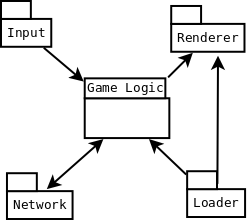
\includegraphics[scale=1]{zasoby/rozdzial3/budowa}
  \caption{Komponenty gry wraz z przepływem danych pomiędzy nimi.}
  \label{fig:multiplayer}
\end{figure}

Dokładniejsze omówienie implementacji poszczególnych komponentów w grze WebArena znajduje
się w rozdziale \ref{cha:implementacja}.

\subsection{Współbieżność}
\label{ssec:wspolbieznosc}

Jednym z prostszych sposobów na wykorzystanie współbieżności w grach jest
rozdzielenie pracy różnych podsystemów pomiędzy wątkami. Ten sposób został
wybrany do WebArena, między innymi ze względu na swoją prostotę,
ale również dlatego, że pozwala on zminimalizować punkty synchronizacji
i ilość przesyłanych danych pomiędzy wątkami, co jest bardzo istotne,
biorąc pod uwagę sposób działania Web Workers -- brak współdzielonej
pamięci (rozdział \ref{ssec:webWorkers}). Wadą takiego sposobu jest
niska skalowalność -- jeżeli podsystemy gry zostały podzielone na dwa
wątki, użytkownik posiadający czterordzeniowy procesor nie zyska
dodatkowego przyśpieszenia. Mimo wszystko, nawet rozdzielenie pracy
pomiędzy dwa rdzenie powinno dać znaczące przyśpieszenie.

W przypadku WebArena podział wygląda następująco:
\begin{itemize}
\item wątek główny -- renderer, obsługa wejścia, pomniejsze podsystemy,
\item Web Worker -- logika gry, synchronizacja sieciowa.
\end{itemize}

Z powodu ograniczeń Web Workers, większość podsystemów bezpośrednio odwołujących
się do zewnętrznych API (np. WebGL, HTML DOM itd.), musi pracować w wątku głównym.
Dodatkowo podczas wczytywania zasobów uruchamiane są dodatkowe wątki do
czasochłonnego parsowania plików, które mogłoby pogorszyć responsywność
aplikacji.

\begin{figure}[h]
  \centering
  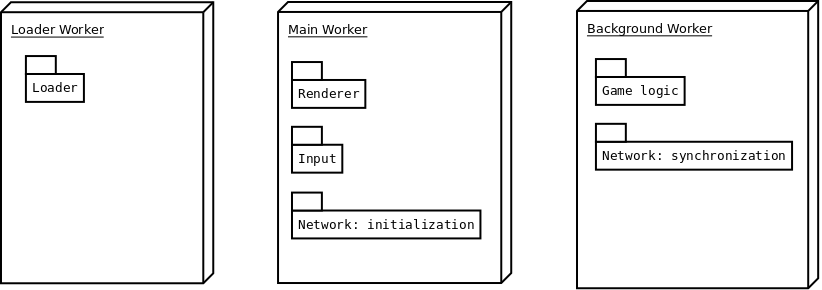
\includegraphics[scale=0.4]{zasoby/rozdzial3/workers}
  \caption{Podział komponentów gry pomiędzy wątki.}
  \label{fig:workers}
\end{figure}

Schemat \ref{fig:workers} przedstawia rozmieszczenie komponentów gry pomiędzy Web
Workery. Jak widać, warstwa sieciowa została rozdzielona na dwie części. Ponieważ
API WebRTC jest dostępne tylko dla głównego wątku, część odpowiedzialna za
nawiązanie i utrzymywanie połączenia sieciowego działa na nim. Część odpowiedzialna
za synchronizację, współdzieli pamięć z logiką gry, dlatego pracuje na drugim
wątku. Komponenty pomiędzy workerami komunikują się tylko za pomocą przesyłanych
wiadomości.

Dyskusję na temat współbieżności w grach i różnych podejść do niej można znaleźć
między innymi w \cite{game-engine}, \cite{multithreaded-game-engine}
i \cite{parallel-game-engine}.

Więcej szczegółów na temat implementacji wielowątkowości w grze WebArena znajduje
się w rozdziale \ref{sec:wielowatkowosc}.

\section{Architektura sieciowa}
\label{ssec:architekturaSieciowa}

Jako, że WebArena jest systemem rozproszonym, należy również omówić architekturę
sieciową gry jako całego systemu -- role urządzeń sieciowych biorących udział w
jego budowaniu.

\begin{figure}[h]
  \centering
  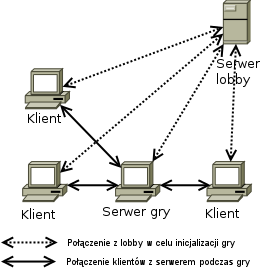
\includegraphics[scale=1]{zasoby/rozdzial2/multiplayer}  
  \caption{Architektura sieciowa gry.}
  \label{fig:multiplayer}
\end{figure}

Serwer lobby pełni jednocześnie dwie funkcje:
\begin{itemize}
\item jest serwerem HTTP hostującym kod źródłowy gry w JavaScript i pliki z
  zasobami gry,
\item jest serwerem Web Sockets, przekazującym pakiety pomiędzy klientami
  i serwerem w początkowej fazie nawiązywania połączenia.
\end{itemize}

Kod serwera jest bardzo prosty i właściwie ogranicza się do statycznego
serwowania plików oraz pasywnego przekazywania pakietów pomiędzy klientami
i serwerem, w celu nawiązania połączenia WebRTC. Z tego powodu serwer
sieciowy nie będzie tutaj szerzej omawiany.

Zgodnie z treścią rozdziału \ref{ssec:multiplayer}, klient oraz serwer gry
są aplikacją działającą w przeglądarce internetowej.



%%% Local Variables: 
%%% mode: latex
%%% TeX-master: "praca"
%%% End: 
